\documentclass[conference]{IEEEtran}
\IEEEoverridecommandlockouts
\usepackage{cite}
\usepackage{amsmath,amssymb,amsfonts}
\usepackage{algorithmic}
\usepackage{graphicx}
\usepackage{textcomp}
\usepackage{xcolor}
\usepackage{array}
\usepackage{enumitem}
\usepackage{siunitx}
\usepackage[spanish]{babel}
\usepackage{multirow}
\usepackage{float}
\usepackage{booktabs}
\usepackage[hidelinks]{hyperref}
\usepackage{hhline}
\usepackage[left=2cm,right=2cm,top=2cm,bottom=2cm]{geometry}
\usepackage{listings}
\usepackage{xcolor}
\usepackage{xurl}

\lstset{
    language=C,
    basicstyle=\ttfamily\footnotesize,
    frame=single,
    breaklines=true,
    breakatwhitespace=false,
    columns=fullflexible,
    keepspaces=true,
    captionpos=b,
    showstringspaces=false,
    tabsize=4,
    aboveskip=1em,
    belowskip=1em
}

\def\BibTeX{{\rm B\kern-.05em{\sc i\kern-.025em b}\kern-.08em
    T\kern-.1667em\lower.7ex\hbox{E}\kern-.125emX}}
    
\begin{document}

\title{Título del informe\\
{\footnotesize \textsuperscript{}}
\thanks{}
}

\author{\IEEEauthorblockN{1\textsuperscript{st} Autor 1}
\IEEEauthorblockA{\textit{Carrera o Departamento} \\
\textit{Universidad o Institución}\\
Ciudad, País \\
correo1@ejemplo.com}
\and
\IEEEauthorblockN{2\textsuperscript{nd} Autor 2}
\IEEEauthorblockA{\textit{Carrera o Departamento} \\
\textit{Universidad o Institución}\\
Ciudad, País \\
correo2@ejemplo.com}
}

\maketitle

\begin{abstract}
% --- Escribe aquí tu resumen ---
\end{abstract}

\textit{Palabras clave:} palabra1, palabra2, palabra3, palabra4

\begin{table}[H]
\centering
\caption{Tipo de implementación por cada parte del Laboratorio 3}
\begin{tabular}{@{}ccc@{}}
\toprule
\textbf{Parte} & \textbf{Tema} & \textbf{Tipo} \\ \midrule
A & Plotter & Física \\
B & Control de temperatura & Simulada y Física \\
C & Control de motor & Simulada y Física \\
D & Matriz RGB & Física \\
E & Cerradura RFID & Simulada y Física \\
F & Mini fútbol & Física \\ \bottomrule
\end{tabular}
\label{tab:implementacion_lab3}
\end{table}

% Plotter


\section{Introducción}

\subsection{Propósito del laboratorio}

\subsection{Objetivos}

\textbf{Objetivo general:}


\textbf{Objetivos específicos:}


\subsection{Descripción general de los módulos}

El laboratorio se divide en seis implementaciones principales:



\subsection{Competencias desarrolladas}

\section{Marco teórico}

\section{Modulación por Ancho de Pulso (PWM)}

La \textbf{Modulación por Ancho de Pulso (PWM, por sus siglas en inglés)} es una técnica utilizada para controlar la potencia entregada a una carga mediante una señal digital.  
Consiste en variar el \textit{ciclo de trabajo} (\textit{duty cycle}) de una onda cuadrada de frecuencia fija.  
El ciclo de trabajo se define como la proporción de tiempo que la señal permanece en nivel alto durante un período completo (\( D = \frac{t_{ON}}{T} \times 100\% \)).  
De esta manera, el valor medio de la tensión aplicada a la carga depende directamente del ciclo de trabajo.

\subsection{PWM en el ATmega328P}

El microcontrolador \textbf{ATmega328P} posee tres temporizadores capaces de generar señales PWM por hardware:

\begin{itemize}
    \item \textbf{Timer0:} de 8 bits — pines de salida \texttt{OC0A} (PD6) y \texttt{OC0B} (PD5).
    \item \textbf{Timer1:} de 16 bits — pines de salida \texttt{OC1A} (PB1) y \texttt{OC1B} (PB2).
    \item \textbf{Timer2:} de 8 bits — pines de salida \texttt{OC2A} (PB3) y \texttt{OC2B} (PD3).
\end{itemize}

Cada uno de estos temporizadores puede configurarse en distintos modos de operación definidos por los bits \texttt{WGMn[3:0]} (Waveform Generation Mode).  
Los modos más utilizados para la generación de PWM son:

\begin{enumerate}
    \item \textbf{Modo Fast PWM:} genera una señal de frecuencia constante y permite variar el ciclo de trabajo modificando el registro \texttt{OCRnx}. Este modo es ideal para control de motores, servos o regulación de brillo en LEDs.
    \item \textbf{Modo Phase Correct PWM:} genera una onda simétrica, variando su ciclo de trabajo de manera que la frecuencia de la señal se reduce a la mitad de la del modo Fast PWM. Se utiliza cuando se requiere una salida con menor distorsión.
    \item \textbf{Modo Normal:} el temporizador simplemente cuenta desde cero hasta su valor máximo (255 u 65535) y reinicia, sin generar una forma de onda PWM.
\end{enumerate}

\subsection{Configuración de registros}

El funcionamiento del PWM depende principalmente de tres registros:

\begin{itemize}
    \item \textbf{\texttt{TCCRnA} y \texttt{TCCRnB}}: determinan el modo de operación (bits \texttt{WGMn}) y la conexión de la salida de comparación (\texttt{COMnx}).
    \item \textbf{\texttt{OCRnx}}: define el valor de comparación que fija el ciclo de trabajo.
    \item \textbf{\texttt{TCNTn}}: contiene el valor actual del contador del temporizador.
\end{itemize}

En modo \textbf{Fast PWM}, la salida cambia de estado cuando el contador \texttt{TCNTn} iguala el valor de \texttt{OCRnx}, reiniciándose al alcanzar su valor máximo.  
En el modo \textbf{Normal}, el contador simplemente incrementa sin modificar ninguna salida, siendo útil para mediciones o temporizaciones.

\begin{figure}[H]
    \centering
    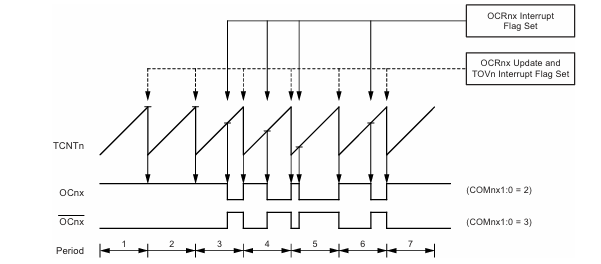
\includegraphics[width=0.35\textwidth]{anexos/Marco Teorico/Fast PMW.png}
    \caption{Diagrama de funcionamiento del modo Fast PWM en el ATmega328P. La señal de salida cambia cuando el contador alcanza el valor de comparación.}
    \label{fig:fast_pwm}
\end{figure}

\begin{figure}[H]
    \centering
    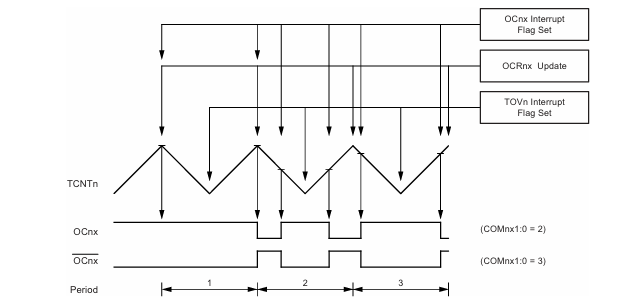
\includegraphics[width=0.35\textwidth]{anexos/Marco Teorico/Phase Correct.png}
    \caption{Modo Normal de operación del temporizador. El contador incrementa hasta su valor máximo y luego se reinicia, sin modificar las salidas.}
    \label{fig:normal_mode}
\end{figure}

\subsection{Aplicaciones}

La modulación PWM es ampliamente utilizada en sistemas embebidos, especialmente para:
\begin{itemize}
    \item Control de velocidad de motores de corriente continua.
    \item Regulación de intensidad luminosa en LEDs.
    \item Control de servomotores (por ejemplo, SG90).
    \item Conversión digital-analógica por filtrado de la señal PWM.
\end{itemize}

En este trabajo práctico, el modo \textbf{Fast PWM} del \texttt{Timer0} se empleó para controlar tanto la potencia disipada en los transistores TIP31 como la velocidad del ventilador mediante el ajuste dinámico del ciclo de trabajo.


\section{Metodología}

\subsection{Materiales y Herramientas}

\begin{itemize}
    \item 
\end{itemize}



\subsection{Procedimiento general}

\subsubsection{Plotter} ---
El sistema del plotter tiene como objetivo controlar de manera coordinada dos motores paso a paso y una válvula solenoide utilizando el microcontrolador ATmega328P. A través de la interfaz serial (UART), el usuario puede seleccionar distintas figuras predeterminadas —como triángulos, cruces o círculos— para su trazado automático. El microcontrolador envía las órdenes de dirección y activación al sistema de potencia, asegurando que los movimientos se mantengan dentro de los límites definidos por los sensores de fin de carrera. De esta forma, el dispositivo permite realizar dibujos controlados en los ejes X e Y, integrando comunicación serial, control de motores y manejo de periféricos en una aplicación práctica de control embebido.

\vspace{1em}

El programa implementa el control completo de un \textit{plotter} didáctico de dos ejes (X e Y) utilizando motores paso a paso y un solenoide que sube o baja el lápiz para dibujar figuras a partir de trayectorias predefinidas almacenadas en memoria de programa (\texttt{path\_data.h}). Emplea interrupciones externas para los finales de carrera (PD2 y PD3), junto con un sistema de antirrebote basado en el temporizador \texttt{Timer0}, que asegura lecturas estables. La función principal inicializa los periféricos y ejecuta de forma secuencial distintas trayectorias (murciélago, círculo, flor, cruz y triángulo), repitiendo el ciclo de dibujo. Cada trayectoria se realiza mediante la función \texttt{execute\_path()}, que mueve los motores de acuerdo con los desplazamientos definidos, controlando dirección y cantidad de pasos en cada eje, mientras el solenoide indica cuándo dibujar. Si un límite se activa, el sistema detiene el movimiento mediante \texttt{emergency\_stop()}, garantizando seguridad. En conjunto, el código conforma un sistema de control secuencial de dibujo automático con soporte para trayectorias reflejadas y detección de límites mecánicos.


\vspace{1em}
\subsubsection{Temperatura} ---
Este módulo mide la temperatura ambiente mediante un sensor LM35 y ajusta automáticamente el funcionamiento de un calefactor y un ventilador según el rango térmico detectado. El ATmega328P ejecuta lecturas periódicas a través del ADC y determina las acciones de control utilizando salidas digitales y señales PWM. El sistema comunica los valores y estados por UART, e incluye un menú que permite modificar el punto medio de temperatura. Además, se prevé una simulación y una implementación física del sistema, complementadas con una gráfica de evolución de temperatura generada en Python o MATLAB.

\vspace{1em}

El programa implementa un sistema de \textbf{control automático de temperatura} utilizando un microcontrolador ATmega328P, un sensor \textit{LM35} para la medición analógica de temperatura y un \textit{ventilador controlado por PWM}. La lectura del sensor se realiza mediante el módulo ADC, y el valor obtenido se convierte a grados Celsius para ser comparado con los umbrales configurables \( t_{C2} \) (mínimo) y \( t_{C3} \) (máximo). Si la temperatura medida excede el rango establecido, el ventilador se activa o desactiva automáticamente. La comunicación con el usuario se realiza a través de la interfaz \textit{UART}, permitiendo visualizar la temperatura, modificar los límites y controlar el sistema mediante comandos como \texttt{Encender}. El programa utiliza interrupciones por temporizador para realizar mediciones periódicas y \textit{buffers} circulares para gestionar la comunicación serial de forma no bloqueante. En conjunto, el sistema presenta un funcionamiento modular, estable y adaptable a diferentes condiciones térmicas.


\vspace{1em}
\subsubsection{Motor} ---
En este sistema se comparan las lecturas de dos potenciómetros, uno como referencia y otro acoplado al eje de un motor, con el fin de igualar ambas señales. El microcontrolador utiliza el conversor ADC para leer los valores y genera una señal PWM que ajusta la velocidad y el sentido de giro del motor hasta lograr la coincidencia. Durante el proceso, se transmiten por UART los valores de referencia, posición actual, nivel de PWM y sentido de giro, permitiendo un seguimiento en tiempo real. El sistema se implementa tanto en simulación como físicamente, complementado con una visualización gráfica de los resultados.

\vspace{1em}

El programa implementa el \textbf{control de posición de un motor de corriente continua} con retroalimentación analógica, utilizando el microcontrolador \textit{ATmega328P}. El sistema compara en tiempo real dos señales analógicas leídas por el ADC: una de referencia (posición deseada) y otra proveniente del potenciómetro acoplado al motor (posición actual). En función de la diferencia o \textit{error}, el microcontrolador ajusta la dirección de giro mediante los pines \texttt{IN1} e \texttt{IN2}, y genera una señal PWM proporcional en \texttt{OCR1A} para regular la velocidad. Se establece una \textit{zona muerta} para evitar oscilaciones y se limitan los valores mínimos y máximos de PWM. Además, el sistema transmite por \textit{USART} los valores de referencia, posición real y salida PWM, junto con la dirección de movimiento, permitiendo el monitoreo en tiempo real desde un ordenador. El procesamiento principal se ejecuta dentro de un bucle que llama periódicamente a la función \texttt{usart\_task()}, mientras las interrupciones gestionan la comunicación serial mediante \textit{buffers} circulares no bloqueantes.


\vspace{1em}
\subsubsection{Matriz} ---
El sistema emplea un joystick analógico para desplazar un LED activo dentro de una matriz RGB, utilizando el ADC del ATmega328P para detectar los movimientos sobre los ejes X e Y. Los límites de desplazamiento están restringidos al área visible de la matriz, y al presionar el botón del joystick se cambia aleatoriamente el color del LED activo. Se incorpora una zona muerta para evitar lecturas erráticas por ruido analógico, garantizando un control preciso y fluido. Esta parte se desarrolla únicamente de forma física en el laboratorio.

\vspace{1em}

El programa implementa un sistema de \textbf{control interactivo de una matriz de LEDs WS2812} (64 píxeles dispuestos en una cuadrícula de 8×8) utilizando el microcontrolador \textit{ATmega328P}, un \textit{joystick analógico} y un \textit{botón con antirrebote}. El joystick controla la posición de un píxel encendido dentro de la matriz (variables \texttt{x\_pos} y \texttt{y\_pos}), mientras que el botón genera colores aleatorios mediante una rutina de interrupción con \textit{debounce}. La comunicación serial \textit{USART} (reutilizada del laboratorio 2) permite monitorear el sistema o enviar datos de depuración. Para generar las señales temporizadas requeridas por los LEDs WS2812, se emplean rutinas en ensamblador inline con \texttt{asm volatile}, asegurando los ciclos exactos por bit. Además, el código utiliza interrupciones por temporizador para contar milisegundos (\texttt{millis\_counter}) y gestionar el antirrebote por software. En conjunto, el sistema integra control analógico, comunicación serial y temporización precisa para crear una interfaz visual interactiva sobre una matriz RGB.


\vspace{1em}
\subsubsection{Cerradura} ---
La cerradura electrónica implementa un sistema de autenticación mediante tarjetas RFID RC522 controladas por el microcontrolador ATmega328P. El identificador único (ID) de la tarjeta autorizada se almacena en la memoria EEPROM para su verificación permanente. La interfaz incluye una pantalla LCD I2C, LEDs indicadores y comunicación UART para mensajes informativos y supervisión externa. El sistema permite registrar, actualizar y eliminar tarjetas de acceso, combinando almacenamiento no volátil, comunicación serie y periféricos de entrada/salida en un diseño de seguridad embebido. Este módulo se desarrolla tanto en simulación como en implementación física.

El programa implementa un sistema de \textbf{control de acceso mediante RFID} con visualización en pantalla LCD e interfaz serial, utilizando el microcontrolador \textit{ATmega328P} y el módulo \textit{MFRC522} para la lectura de tarjetas. El sistema cuenta con tres modos principales: verificación de acceso, registro de una nueva tarjeta y borrado del UID almacenado. Los identificadores se guardan de forma persistente en la memoria \textit{EEPROM}, y se comparan con los leídos en tiempo real. La interacción del usuario se realiza tanto por medio de la comunicación \textit{UART} como mediante botones físicos conectados al puerto C. La información de estado se muestra en una pantalla LCD controlada por interfaz \textit{I2C} (expansor PCF8574), mientras que un buzzer emite alertas acústicas en casos de acceso denegado o eventos relevantes. Internamente, el sistema utiliza comunicación \textit{SPI} para el módulo RFID, \textit{I2C} para el LCD y \textit{USART} con buffers circulares para comunicación no bloqueante. En conjunto, el código integra múltiples periféricos y subsistemas (SPI, I2C, UART, EEPROM e interrupciones) para construir un sistema embebido completo y robusto de autenticación electrónica.


\vspace{1em}
\subsubsection{Fútbol} ---
Esta consigna consiste en el diseño y programación de un robot móvil basado en el ATmega328P, capaz de disputar partidos de mini fútbol sobre un campo reducido. El robot integra sensores, actuadores y sistemas de comunicación inalámbrica (Bluetooth o RF) para detectar y conducir el balón hacia la portería rival. Se evalúan la autonomía, el control, la integración mecánica y la creatividad del diseño. Este proyecto se realiza únicamente de forma física, siendo el cierre práctico y competitivo del laboratorio.

\section{Resultados}


\subsection{Resultados por módulo}


\subsection{Temperatura}
El circuito final de esta consigna del laboratorio se puede ver en la imagen correspondiente. 

\paragraph{Envío de datos por USART}

En la Figura \ref{fig:Tem_USART} se puede observar la forma en la que se enviaban los datos por puerto serial entre el \texttt{ATmega328P} y el código de Python. 

\begin{figure}[H]
    \centering
    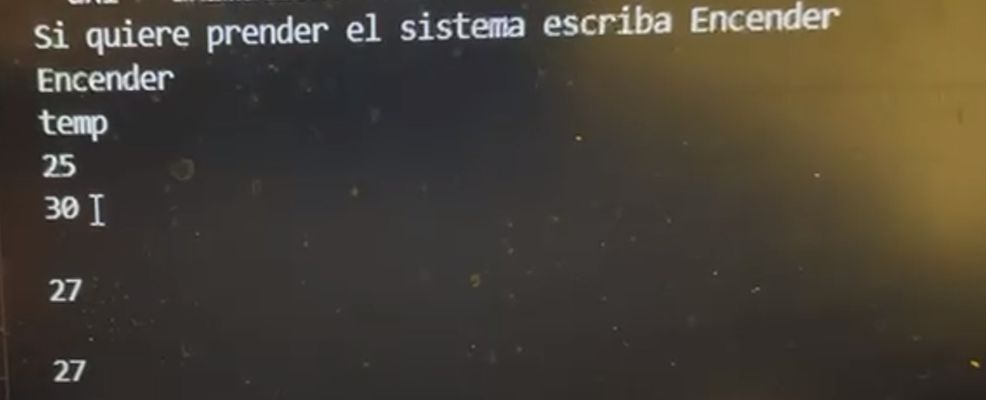
\includegraphics[width=0.35\textwidth]{anexos/2 Temperatura/USART Temperatura.png}
    \caption{Comunicación de datos vía USART entre el microcontrolador y Python.}
    \label{fig:Tem_USART}
\end{figure}

\paragraph{Gráfica en tiempo real}

El resultado de la gráfica en tiempo real se muestra en la Figura \ref{fig:Grafica1}. En ella se observa cómo el eje X representa la evolución temporal de la ejecución (hora de registro en tiempo real), mientras que en el eje Y se visualizan los valores de temperatura obtenidos cada segundo.  
Además, se incluye una línea de referencia que indica la temperatura media esperada.

\begin{figure}[H]
    \centering
    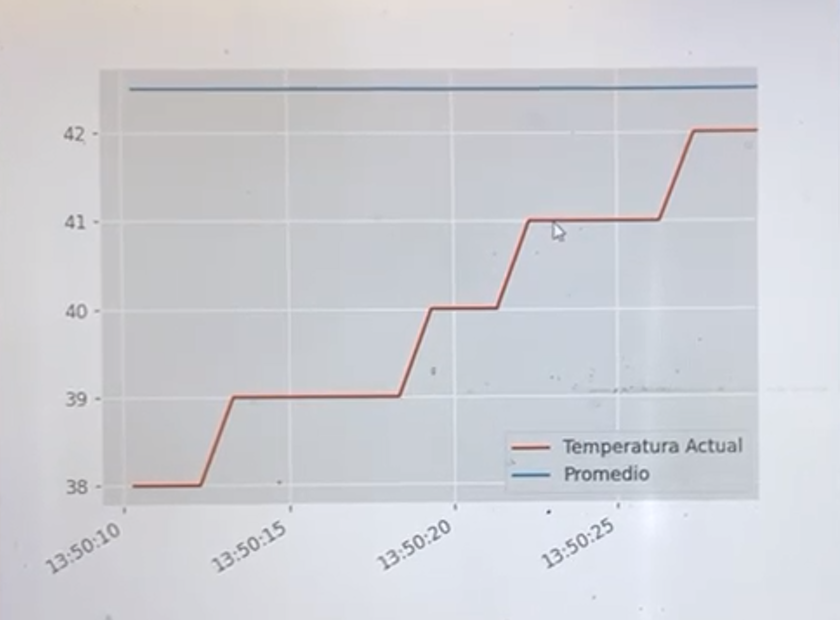
\includegraphics[width=0.35\textwidth]{anexos/2 Temperatura/Grafica tiempo real.png}
    \caption{Gráfica de temperatura en tiempo real.}
    \label{fig:Grafica1}
\end{figure}

\paragraph{Simulación}

Véase la Figura  para una representación del montaje de la simulación, la cual fue realizada en el entorno \textbf{Proteus}. En dicha figura se puede observar la disposición de los componentes utilizados y las conexiones correspondientes al sistema de control térmico.

\paragraph{Gráfica de la simulación}

El resultado de la gráfica correspondiente a la simulación se muestra en la Figura .  
De manera análoga a la gráfica en tiempo real, se presentan en una misma figura tanto la temperatura de referencia como la temperatura medida en cada instante de tiempo.  
La diferencia principal radica en que en esta gráfica se visualiza la **línea temporal completa** de toda la simulación.

\section{Conclusiones}
\subsection{Reflexiónes individuales}

    \subsubsection{Plotter}
    % El plotter funciono bien
    % La cagada fue el juego de la estructura
    % A veces se trancaba y hacia cualquier cosa
    % Hubiera estado bueno tener USART para poder tener feedback del sistema
    % Mejoras: 
    %   Optimizar el programa de trazos para que ocupe menos espacio
    %   Aumentar la velocidad de dibujo sin comprometer el trazado de las figuras.
    %   Reparar la estructura del plotter para evitar trancasos.
    
    \subsubsection{Temperatura}

   % La implementacion del control de Temperatura ocn el modulo que incluia un calentador y el ventilador, fue stisfactoria. Se cumplieron correectamente los objetivos buscados. Se puede mejorar incluyendo un control pmw segun la diferencia de temperatura al calentador, no solo en el ventilador. 
  %  Asi como incluir en la grafica el estado de los perifericos del sistema, el ventilador y el calentador, si esta encendido o no. 
    teamohector
    \subsubsection{Motor}
    % El motor funciono bien, tuvo una buena respuesta a movimientos suaves y bruzcos, y lograba estabilizarse correctamente sin oscilaciones.
    % Lo que se pudo haber mejorado era reducir la zona muerta para tener una mejor precision
    % al momento de realizar movimientos pequeños. 
    
    \subsubsection{Matriz}
    % La matriz funciono bien, reconoció bien las entradas del joystick. Al trabajar solamente con la saturacion de los potenciometros, lo que se pudo haber mejorado era que el punto se moviera a diferentes velocidades dependiendo de la posición del joystick.

    \subsubsection{Cerradura}

   % Funciono correctamente, teniendo una correta comunicacion via spi entre el esclavo (RC522) y el maestro(Arduino), permitio entender correctamente como funciona ese tipo de comunicacion. A su vez tambien una correcta sincronizacion con la pantalla LCD via I2C. Se podria haber hecho mas satisfactorio y enriquecedor, ncluyendo la opcion de modificar las tarjetas RFID.


\subsection{Reflexión general}



\bibliographystyle{IEEEtran}
\nocite{*}
\bibliography{5_referencias}

\appendix
\section{Anexos}

\subsection{Drive de Laboratorio}
La carpeta de Google Drive correspondiente a este laboratorio puede encontrarse en \url{https://drive.google.com/drive/folders/1fylHKdJC3ad7wB_ZZz2fyQ-oS7G_49QM?usp=sharing}. Allí encontrará evidencias del trabajo realizado durante esta actividad.

\subsection{Fragmentos de codigo}

\subsubsection{\textbf{Plotter}}---
\paragraph{Configuracion de USART}\label{anexo:config_USART}---\\
\begin{lstlisting}[language=C, caption={Configuracion de USART}]
// Code here
\end{lstlisting}

\paragraph{Configuracion de USART}\label{anexo:PMW_Temperatura}---\\
\begin{lstlisting}[language=C, caption={Configuracion de PMW para la temperatura}]
// D6 (PD6/OC0A) con Timer0
// D11 (PB3/OC2A) con Timer2
void Init_pwm(void){
	// --- Salidas PWM ---
	DDRD |= (1 << DDD6);   // D6 = OC0A
	DDRB |= (1 << DDB3);   // D11 = OC2A
	//PORTB |= (1 << PORTB3);

	// ---- Timer0: Fast PWM 8-bit, no inversor en OC0A, N=64 (~976 Hz) ----
	TCCR0A = (1 << WGM01) | (1 << WGM00)| (1 << COM0A1);               // OC0A no inversor (D6)
	TCCR0B = (1 << CS01)  | (1 << CS00);  // N=64
	OCR0A  = 0;                           // duty D6

	// ---- Timer2: Fast PWM 8-bit, no inversor en OC2A, N=64 (~976 Hz) ----
	TCCR2A = (1 << WGM21) | (1 << WGM20)| (1 << COM2A1);               // OC2A no inversor (D11/PB3)
	TCCR2B = (1 << CS22);                 // CS22:CS21:CS20 = 100 => N=64
	OCR2A  = 0;                           // duty D11
}
\end{lstlisting}


\paragraph{Configuracion de USART}\label{anexo:DeltaTemp_Ventilador}---\\
\begin{lstlisting}[language=C, caption={Control de velocidad del ventilador}]
		uint8_t d_t   = (int8_t)tC - (int8_t)(tC3);
		uint8_t pwm2;
		if(d_t > 0){
			
			if (d_t > 20)       pwm2 = 255;
			else if (d_t > 10)  pwm2 = 125;
			else if (d_t > 5)   pwm2 = 50;
			else                pwm2 = 25;

			OCR2A = pwm2;   
		}
		
\end{lstlisting}



\end{document}
